\section{Pesquisas do Gartner}

A seguir, apresentamos alguns estudos do Gartner (líder mundial na
pesquisa de tecnologia de informação que também atua como empresa de consultoria):

\begin{itemise}

    \item Aproximadamente 19\% das organizações ao redor do mundo estão utilizando a
    computação em nuvem para produção de aplicações, enquanto outros 20\% contratam
    serviços públicos de armazenamento na nuvem. O principal modelo sendo utilizado é
    a da nuvem híbrida~\cite{gartner-public-cloud-services}.

    \item Consumidores armazenarão mais de 1/3 de seu conteúdo digital na nuvem por
    volta de 2016~\cite{gartner-one-third}.

    % Segundo estimativas do grupo americano de informática IBM, o mercado mundial de
    % computação em nuvem poderia alcançar os 200 bilhões de dólares em 2020.

\end{itemise}

Os resultados mostram que a nuvem oferece grandes oportunidades de negócios,
especialmente para serviços de armazenamento. 

Ao mesmo tempo, a indústria de serviços de nuvem é grande e conta com muitos 
provedores com estratégias agressivas para conquistar clientes. Para orientar as 
companhias na hora de selecionar seu parceiro, o Gartner elegeu os dez principais 
fornecedores de serviços de armazenamento~\cite{gartner-top-10}, levando em 
consideração a capacidade deles de atendimento aos clientes:

\begin{figure}[ht]
    \centering
    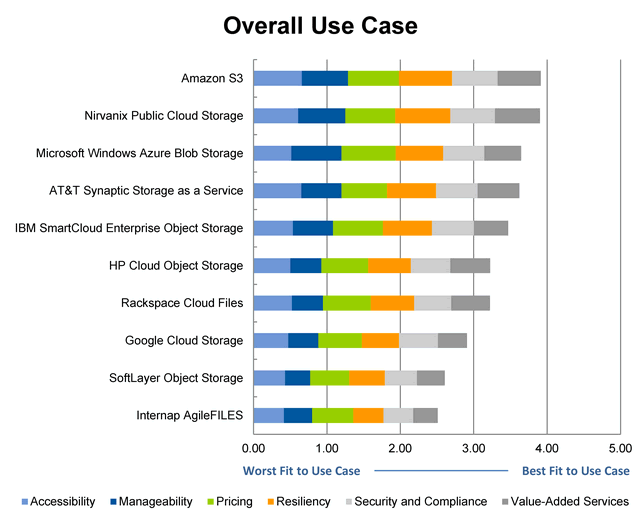
\includegraphics[width=0.9\textwidth]{img/top10.png}
    \caption{Avaliação dos dez principais fornecedores, segundo o Gartner}
\end{figure}
